\documentclass{article}
\usepackage[utf8]{inputenc}
\usepackage{hyperref}
\usepackage[letterpaper, portrait, margin=1in]{geometry}
\usepackage{enumitem}
\usepackage{amsmath}
\usepackage{booktabs}
\usepackage{graphicx}

\usepackage{titlesec}

\titleformat{\section}
{\normalfont\Large\bfseries}{\thesection}{1em}{}[{\titlerule[0.8pt]}]
  
\title{Homework 9}
\author{Ana Mazmishvili}
  
\begin{document}
  
\maketitle

\section{Stata}
\noindent 1.  A yearly plot of the recycling rate for NYC and the controls separately is presented on Figure \ref{fig:NYCNJMA}, while the sum of controls is presented on Figure \ref{fig:NYCvsControls}. 

\begin{figure}[h!]
    \centering
    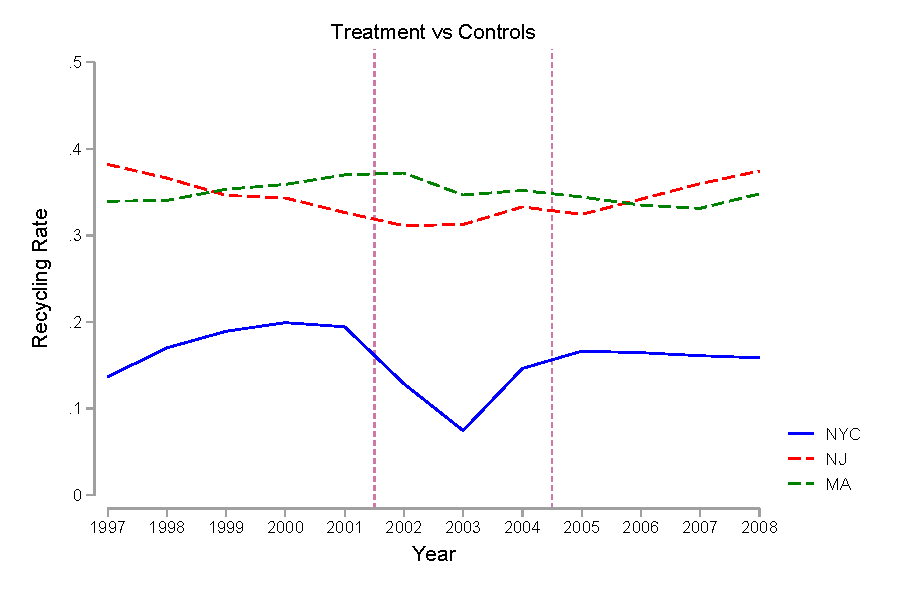
\includegraphics{homework 9/output/figure/treatedvscontrol.pdf}
    \caption{Recycling rate for NYC and the controls}
    \label{fig:NYCNJMA}
\end{figure}

\begin{figure}[h!]
    \centering
    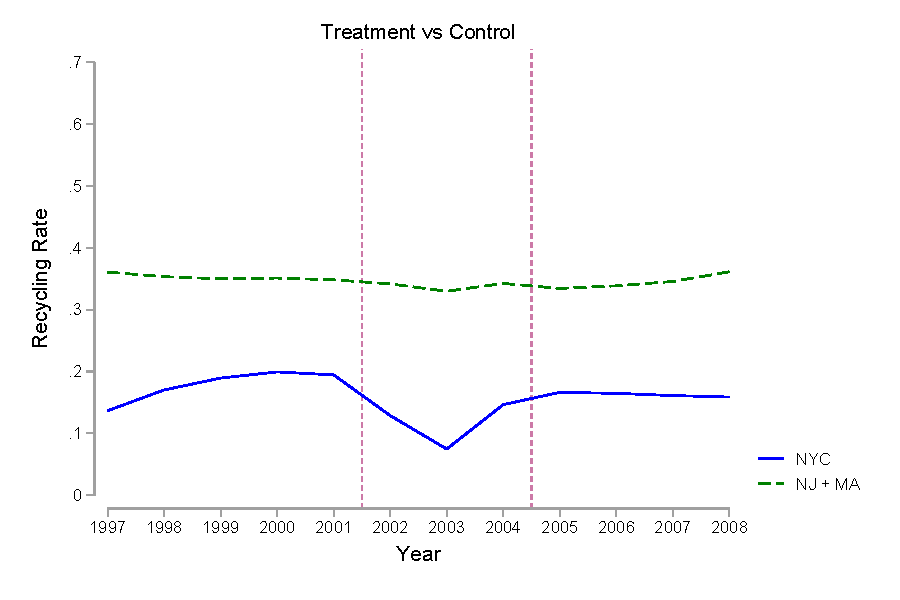
\includegraphics{homework 9/output/figure/linechartrecyclingrate.pdf}
    \caption{Recycling rate for NYC and the sum of controls}
    \label{fig:NYCvsControls}
\end{figure}

\clearpage

\noindent 2. The effect of the pause on the recycling rate in NYC using a TWFE regression and the data
from 1997-2004 is  -.0619874 and the clustered standard error is  .0058221.


\noindent 3. The estimated average treatment effect and the synthetic DID is presented on the Figure \ref{fig:sdid}

\begin{figure}[h!]
    \centering
    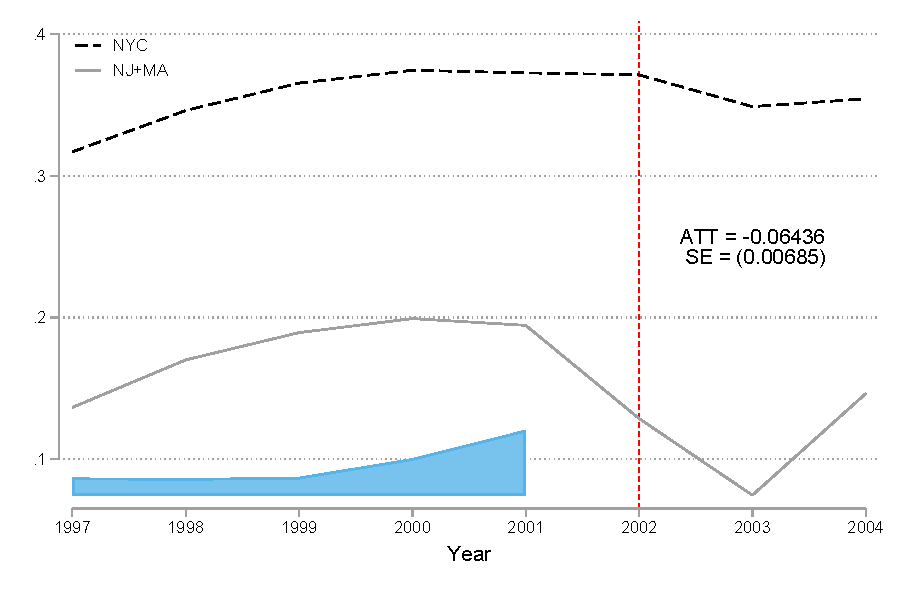
\includegraphics{homework 9/output/figure/sdid.pdf}
    \caption{Average treatment effect and the synthetic DI}
    \label{fig:sdid}
\end{figure}

\clearpage

\noindent 4.  The event study regression results are presented on Figure \ref{fig:ES} 

\begin{figure}[h!]
    \centering
    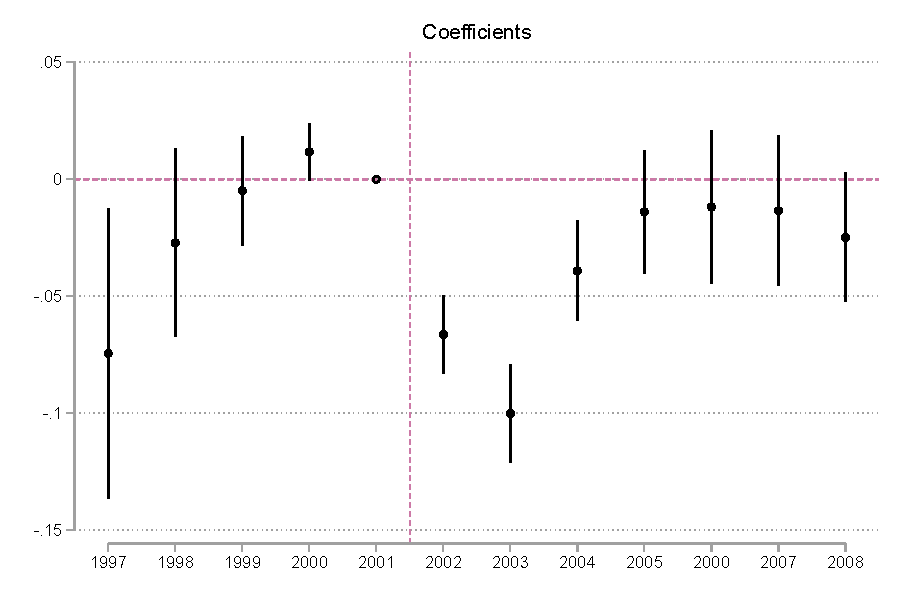
\includegraphics{homework 9/output/figure/eventstudy.pdf}
    \caption{Event Study}
    \label{fig:ES}
\end{figure}

\clearpage
\noindent 5.a The plot of raw outcomes for treated and control groups over time is presented on Figure \ref{fig:raw}.
\begin{figure}[h!]
    \centering
    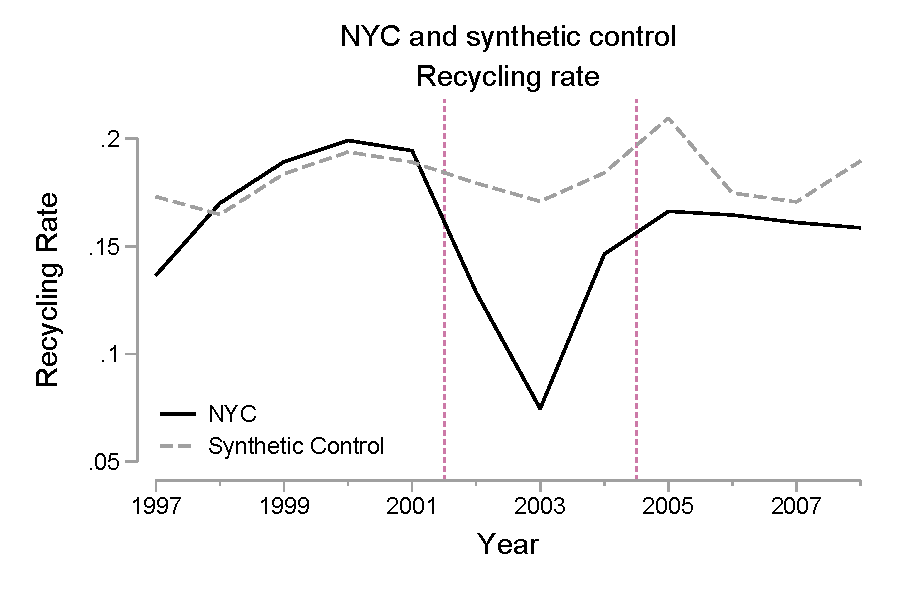
\includegraphics{homework 9/output/figure/scrawoutcomes.pdf}
    \caption{Raw outcomes for treated and control groups}
    \label{fig:raw}
\end{figure}

\clearpage

\noindent 5.b. The plot of raw outcomes for treated group and synthetic control group over time is presented on Figure \ref{fig:SCcontolvstreated}.
\begin{figure}[h!]
    \centering
    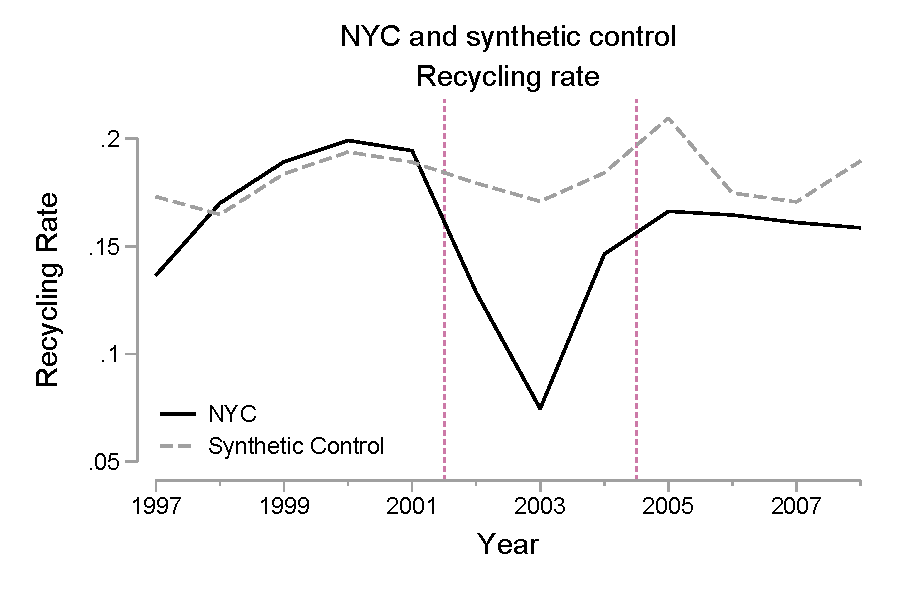
\includegraphics{homework 9/output/figure/sctreatcontrol.pdf}
    \caption{Recycling rate for NYC and the sum of controls}
    \label{fig:SCcontolvstreated}
\end{figure}

\clearpage

\noindent 5.c. The plot of estimated synthetic control effects and placebo effects over time is presented on Figure \ref{fig:placebo}.
\begin{figure}[h!]
    \centering
    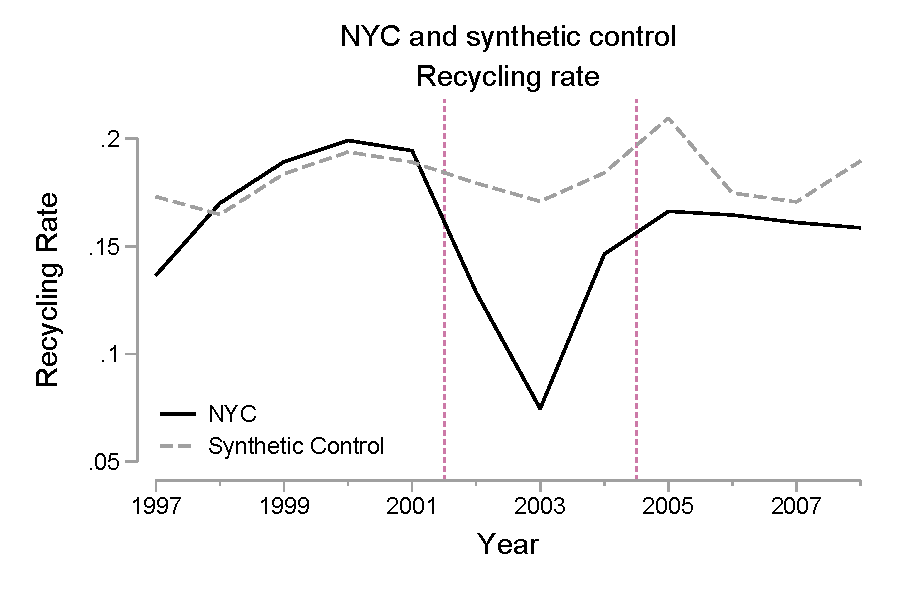
\includegraphics{homework 9/output/figure/scplacebos.pdf}
    \caption{Estimated synthetic control effects and placebo effects}
    \label{fig:placebo}
\end{figure}


\clearpage

\noindent 5.d. The plot of final synthetic control estimates over time is presented on Figure \ref{fig:SCestimates}. 
\begin{figure}[h!]
    \centering
    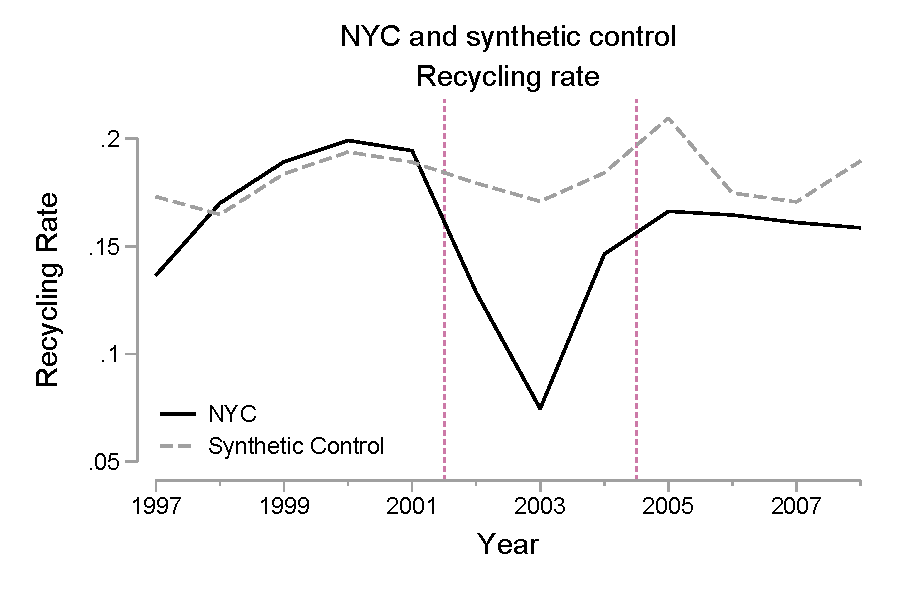
\includegraphics{homework 9/output/figure/scestimates.pdf}
    \caption{Final synthetic control estimates}
    \label{fig:SCestimates}
\end{figure}

\end{document}